\section{Quantum Topics Justification}

\subsection{Motivation \& Teaching Strategy}

Central to an OBTL approach is to ask "what does the student need to be able to do?". 
There is no lack of introductory quantum materials, university course syllabi and online courses available \cite{Ekert:2000}\cite{Abhijith:2022}\cite{Lipton:2021},  
yet exploring every corridor in the labyrinth of quantum topics is not possible within a single module.
Instead we can focus on competencies that matter.

We should reasonably expect that the student be able to accomplish a range of tasks such as:
\begin{itemize}
	\item Explain why and where quantum computers can gain advantage over classical algorithms.
	\item Digest literature by having a familiarity with the standard notations and nomenclatures (Dirac bra-kets, circuit diagrams, complexity metrics).
	\item Assess the suitability of different quantum hardware platforms (superconducting, trapped-ion, photonic, annealing) and highlighting their strengths and weaknesses for different classes of problems.
	\item Demonstrate proficiency with some of the current generation of quantum SDKs.
	\item Gain a mastery over a set of algorithmic building blocks (e.g. state preparation, Quantum Fourier Transform, amplitude amplification) and deploy them on simulated, and preferably real,
	 quantum devices.
	\item Produce meaningful analysis by applying these skills to a novel problem and interpreting the results critically.
\end{itemize}

Drilling into the last point and working backwards, we ask: 
How can we construct focused content that enables students new to quantum computing to master a compact set of 
building blocks with wide applicability, equipping them to tackle more advanced applications
within the limits of an introductory course?

In this section we walk through a set of foundational quantum topics needed to understand, 
and reconstruct, Peter Shor's quantum algorithm for integer factorisation and discrete logarithms.
As we do this, we show how undergraduate-level mathematics and computer-science knowledge 
illuminate how Shor demonstrated the exponential speed up of a classically known algorithm.

We then pull apart his quantum algorithm to reveal the concepts it showcases 
(state preparation, modular arithmetic, the Quantum Fourier Transform, and amplitude amplification) 
each of which has since been generalised into more advanced quantum building blocks that are now used 
across a variety of quantum algorithms.  
Mastering these core concepts provides a toolkit to analyse 
a wider range of beasts in the "quantum zoo"\cite{Jordan:2024}.

The third step in our justification is to walk through a case-study
and back-map the skills required to produce a novel piece of analysis 
to the building-block concepts already identified.

That mapping yields the specific learning outcomes and topic list that is used 
to build our syllabus outline in the next section, thereby providing a clear justification for each topic's inclusion.

%%%%%%%%%%%%%%%%%%%%%%%%%%%%%%%%%%%%%%%%%%%%%%%%%%%%%%%%%%%%%%%%%%%%%%%%%%%%%%%%%%%%%%%%%%%%%%%%%%%%%%%%%%%%%%%%%%%%%%%%
%%%%%%%%%%%%%%%%%%%%%%%%%%%%%%%%%%%%%%%%%%%%%%%%%%%%%%%%%%%%%%%%%%%%%%%%%%%%%%%%%%%%%%%%%%%%%%%%%%%%%%%%%%%%%%%%%%%%%%%%

A meaningful introductory course in quantum computation must maximise the leverage of 
existing classical competencies whilst respecting the varied backgrounds of its students.  
Cloud-based quantum facilities now make hands-on and practical skills attainable; 
nevertheless the field is still steeped in algebraic notations and intricate physical calculus. 
To engage a wider community of engineers and mathematicians,
we focus on the core concepts and mathematical tools required to implement quantum algorithms,
rather than exhaustive theory.

Viewed through a cryptographic lens we see how analogue quantum phenomenon underpin key-distribution protocols,
while Shor's celebrated digital quantum algorithm famously breaks the one-way functions of asymmetric cryptography.
The temptation may be to pivot to the study of post-quantum encryption schemes, 
but we must first understand the quantum computation mechanisms clearly.  

%Why turn-away from cryptographic research areas and look at quantum algorithms more generally?
%The area of understanding new quantum algorithms, and reverse engineering classical algorithms \emph{cite{something}} is burgeoning.
%And the understanding if these new 

%Take, as an example, the \href{https://csrc.nist.gov/CSRC/media/Presentations/crystals-dilithium-round-3-presentation/images-media/session-1-crystals-dilithium-lyubashevsky.pdf}{CRYSTAL-Dilithium NIST "Schnorr-like” lattice-based signature scheme}.
%Schnorr's identification protocol \emph{cite{Schnorr:1990}} 
%\href{https://cybersecurity.springeropen.com/articles/10.1186/s42400-023-00198-1}{is an example a zero-knowledge protocol} 
%that need to convince a verifier knows the discrete logarithm \emph{I may have misunderstood the last point}.
%The hardness assumptions are based on the computational problems of the \emph{Shortest Vector Problem (SVP)} 
%and \emph{Closest Vector Problem (CVP)}.  
%We have jumped from the understanding of quantum phenomenon and promise and pitfalls of quantum technologies to
%a specialised topic in mathematics \emph{what's the best description of the topics around SPV and ZK}.  
%These are interesting a challenging topics, but should be introduced in their own way.

%But moving forward, with the introductory course, into more general quantum algorithms that are not directly applicable to cryptography
%provided it's own benefits.
%Firstly is, the current generation of analogue quantum annealing computers \emph{cite or reference D-Wave} are being used to attempt
%to break certain \emph{Substitution-Permutation Network (SNP)} problems.
%This demonstrates that a working understanding of quantum annealing and QUBO solvers is something that is at least in our bailiwick.
%More simply, we don't know how the next generation of quantum algorithms could be used to attack encryption protocols, 
%so rounding out the programme by looking more generally at these algorithms is justified. 


%%%%%%%%%%%%%%%%%%%%%%%%%%%%%%%%%%%%%%%%%%%%%%%%%%%%%%%%%%%%%%%%%%%%%%%%%%%%%%%%%%%%%%%%%%%%%%%%%%%%%%%%%%%%%%%%%%%%%%%%
%%%%%%%%%%%%%%%%%%%%%%%%%%%%%%%%%%%%%%%%%%%%%%%%%%%%%%%%%%%%%%%%%%%%%%%%%%%%%%%%%%%%%%%%%%%%%%%%%%%%%%%%%%%%%%%%%%%%%%%%
\subsection{Leveraging Classical Competencies}

%\emph{With the varied backgrounds of students we can't assume a core set of mental models, 
%	so don't skip the intro details, but move fast to get everyone up to speed.}

%\emph{This can be aided by leveraging core competencies within the existing curriculum; 
%	presenting a lot of algorithms will have analogies within disciplines already being presented.}

Because students enter with varied backgrounds, we cannot assume shared mental models; 
we therefore start from fundamentals but advance quickly.
Many quantum techniques map directly onto material already covered at the undergraduate level:

\begin{itemize}
	\item \emph{Quantum Machine learning techniques} \cite{Schuld:2014} $\leftarrow$ linear-algebra / kernel methods
	\item \emph{Post-quantum cryptography} \cite{Bernstein:2008} $\leftarrow$ number theory, lattice maths.
	\item \emph{Quantum key distribution} \cite{MummadiFathima:2024} $\leftarrow$ information-theory concepts.
\end{itemize}

To illustrate this bridging strategy, we choose a concrete problem that is likely to motivate newcomers:
quantum kernels for \emph{One-Class Support Vector Machines} (OC-SVMs) used for anomaly detection.
By deconstructing this application, we look to reveal precisely the skills a student must master.
But some mathematical tools of quantum computation (Dirac notation, tensor products, unitary evolution)
are non-negotiable and must be introduced early, though without excessive pedagogy.

This example also underscores the broader point that
effective delivery should draw on competencies already present in the curriculum.
Students should feel confident that they can apply core quantum principals to novel situations.  
The example that will be presented here is of applying familiar notions of time and space complexities 
to estimate quantum-resource requirements.

%%%%%%%%%%%%%%%%%%%%%%%%%%%%%%%%%%%%%%%%%%%%%%%%%%%%%%%%%%%%%%%%%%%%%%%%%%%%%%%%%%%%%%%%%%%%%%%%%%%%%%%%%%%%%%%%%%%%%%%%
%%%%%%%%%%%%%%%%%%%%%%%%%%%%%%%%%%%%%%%%%%%%%%%%%%%%%%%%%%%%%%%%%%%%%%%%%%%%%%%%%%%%%%%%%%%%%%%%%%%%%%%%%%%%%%%%%%%%%%%%
\subsection{Foundational Topics}

Getting a solid grip on the mathematical underpinnings of quantum computation is key, 
and there is a balance between gaining mastery of these necessary skills and casting our net too widely.

%There are examples of introductions to quantum computations that eschew the starting with quantum concepts, 
%Lipton \cite{Lipton:2021}, Abhijith \cite{Abhijith:2022}, Ekert \href{https://arxiv.org/pdf/quant-ph/0011013}{Basic concepts in quantum computation}.
%Nielsen, on the other hand, introduce the concepts of quantum behaviour, the mathematical constructs needed to model these,
%and an application of entanglement in super-dense coding that is a good model to covering ground quickly \cite{Nielsen:2010}

\subsubsection{Digital and Analogue Quantum Computing}

Returning to Feynman's and Deutsch's early quantum computing insights, Feynman was observing that classical machines 
scale badly when simulating quantum-mechanical systems.  
He was suggesting building devices whose own dynamics replicate a \emph{Hamiltonian} of a target quantum system,
to study physical systems such as molecules and condensed-mater models \cite{Feynman:1986}.  
These "analogue" simulators would be highly efficient for a narrow class of problems, 
and have been found to be incredibly powerful in this respect,
but they are not freely programmable.

Deutsch introduced the notion of a universal \emph{digital quantum computer} \cite{Deutsch:1985}; 
a machine that manipulates abstract \emph{qubits} with a gate set, 
much like a classical computer manipulates bits with logic gates.

In today's quantum landscape, we can see both strands being used to tackle new research areas.
Problem‑specific hardware such as D‑Wave annealers \cite{DWave:QuantumAnnealing} 
and Rydberg quantum simulators \cite{Wu:2021}, 
sit along side gate based, programmable processors from IBM \cite{IBM:2016a}, Google \cite{Google:2024a} and others.


%Examples of where natural advantages of certain technologies, such as photonics for quantum communication 
%and quantum cryptography and key distribution can be discussed.

%Photonics poses interesting challenges and opportunities. 
%Is both one of the earliest \emph{cite{photonics}} practical quantum technologies 
%and an expensive one to set up research for \emph{cite{photonics:costs-of-research}}. 
%Yet it has easily demonstrates a number of quantum principles in a way which is easily explainable at an under-graduate science level.
%Early \emph{Quantum Key Distribution (QKD)}  \index{Quantum Key Distribution} used quantum properties of photons, 
%specifically photon polarisation - which can be demonstrated with polarised sunglasses - to develop the delivery of one-time pads 
%for secure communications.

%Further, the exposition of the QKD of randomly generated one time pads highlights another recent development
%where quantum randomness was demonstrated for the first time recently, using digital quantum computers and
%\emph{Random Circuit Sampling} (RCS) \cite{Quantinuum:QRNG}.

%Looking at the physical implementation of quantum systems, we will see certain advantages of different quantum particles
%with respect to  \emph{noise}, \emph{decoherence} and \emph{gate fidelity}.
%This brings into scope the topics of near-term \emph{NISQ} vs the holy-grail of \emph{FTQC}, 
%laying the ground work for the introduction of quantum error correction schemes.


Our syllabus will be focused on those platforms that are cloud based and accessible (gate based digital, analogue annealers, for example), 
but we still introduce a range of quantum computing machinery to understand this landscape.

%%%%%%%%%%%%%%%%%%%%%%%%%%%%%%%%%%%%%%%%%%%%%%%%%%%%%%%%%%%%%%%%%%%%%%%%%%%%%%%%%%%%%%%%%%%%%%%%%%%%%%%%%%%%%%%%%%%%%%%%
\subsubsection{Qubits \& State Spaces}

Starting with some mental models of quantum information and how it is distinct from classical information
and refreshing some linear algebra, matrix manipulation and polar notations will be needed.  
%We don't need to go into in-depth in descriptions of the main quantum particles, but 

We begin with physical intuition of two-level quantum systems, where a quantum particle has two distinct states:
\begin{itemize}
	\item A photon with horizontal or vertical polarization of its electromagnetic field.
	\item An electron with up or down spin state.
	\item A trapped ion with a ground or excited energy state.
\end{itemize}

Laboratory apparatus can prepare and manipulate  the state of these particles.
This mental model gives a base for the core abstraction of quantum information and computation.

\begin{figure}[ht]
	\begin{adjustbox}{center}
		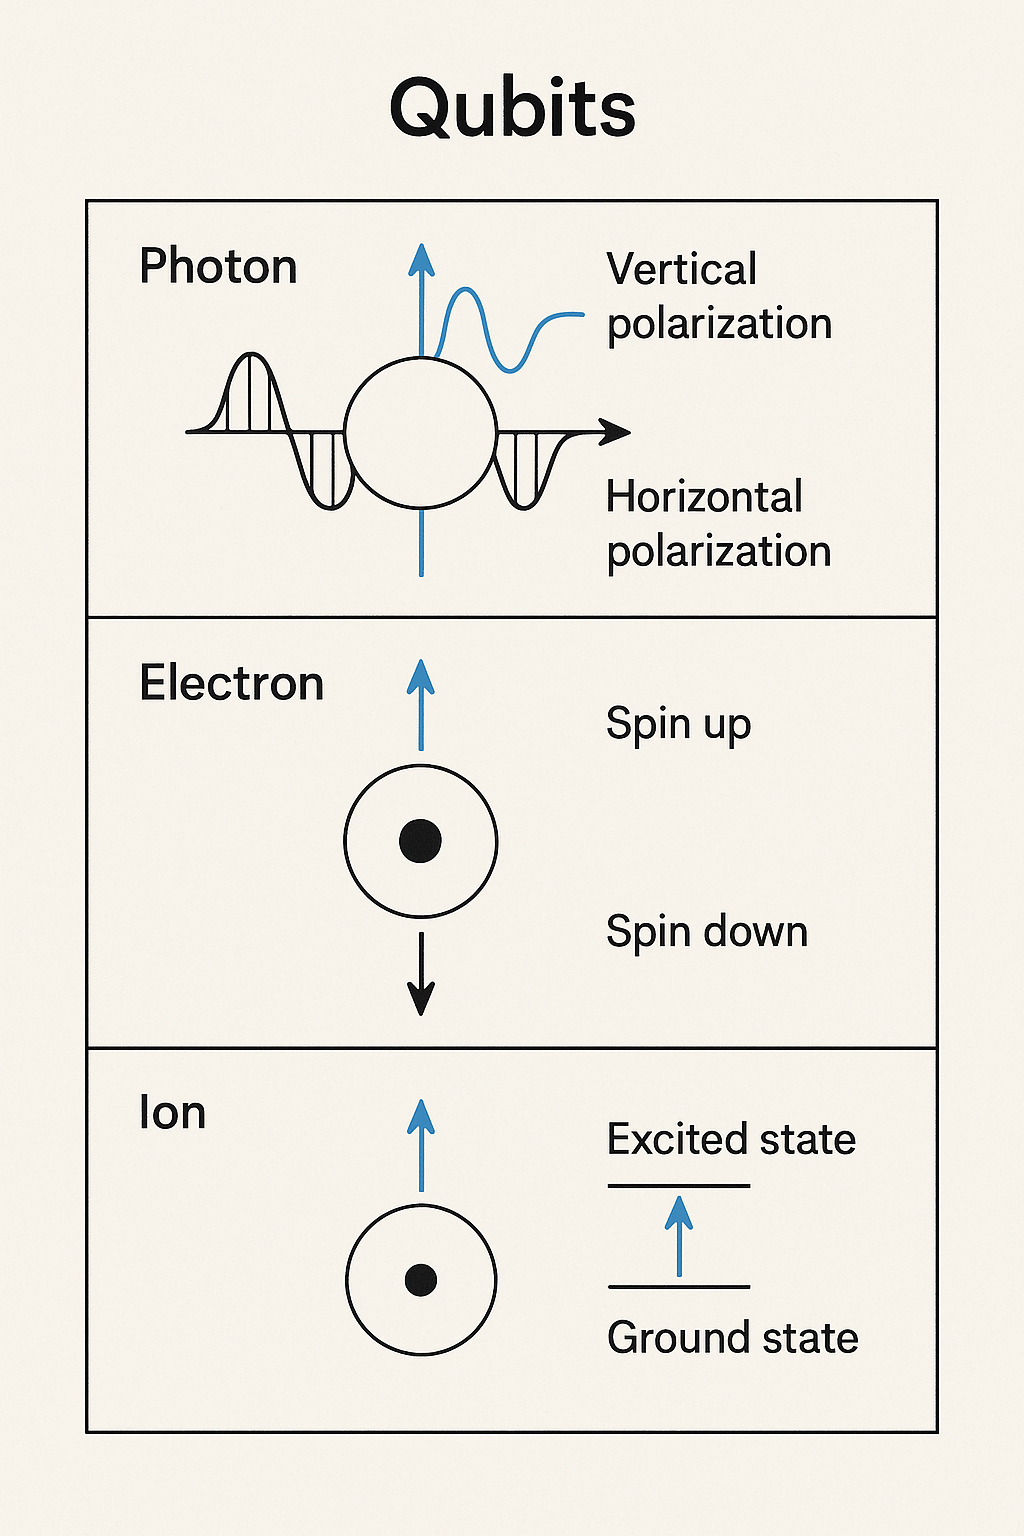
\includegraphics[width=0.4\textwidth, inner]{figures/physical_qubits_2.png}
	\end{adjustbox}
	\vspace{4pt}
	\caption{Representation of physical qubit states} %\href{https://commons.wikimedia.org/wiki/File:Tolmukapea.jpg}{https://commons.wiki-\\media.org/wiki/File:Tolmukapea.jpg}.}
	\label{fig:phys_qubit}
\end{figure}

These simple two level quantum systems have two states that we can label $\lvert0\rangle$ and $\lvert1\rangle$;
"horizontal" or "vertical", "up" or "down", "ground" or "excited".
We can then draw an analogy between a digital bit in a classical computer that has the states $0$ or $1$.
What is different about the information being manipulated in these two systems?

In a digital system we have a switch that we can flip the bit of information from one state to another.

In the quantum system, our quantum bit, or qubit, behaves more like a hi-fi balance knob 
that can be fully in one state or the other, or a mixed, linear, combination of the two states.
This \emph{superposition} of states allows the qubit to encode multiple possibilities simultaneously, 

And this underpins the speed-ups achieved by certain quantum algorithms\cite{Nielsen:2010}.
In this framing, two-level quantum system has an amplitude  $\alpha$ and $\beta$  for each of the states,
and the combined particle state is the vector: 
$$\lvert\psi\rangle = \alpha \lvert0\rangle + \beta \lvert1\rangle $$

Graphically we can represent the combined state of these two special orthogonal \emph{computational basis states} 
as a point on a unit circle in a regular Euclidean space, a generalisation of which is a \emph{Hilbert space}.  

\begin{figure}[ht] 
	\begin{adjustbox}{center}
%		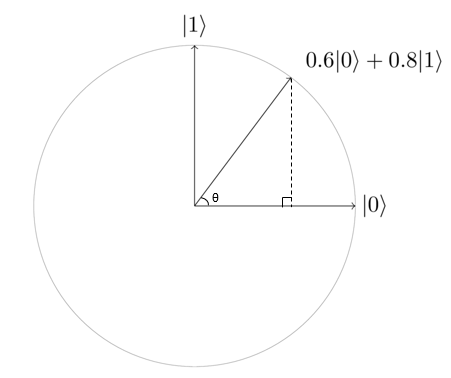
\includegraphics[width=0.5\textwidth, inner]{figures/unit-vector-2-d-hilbert-state.png}
		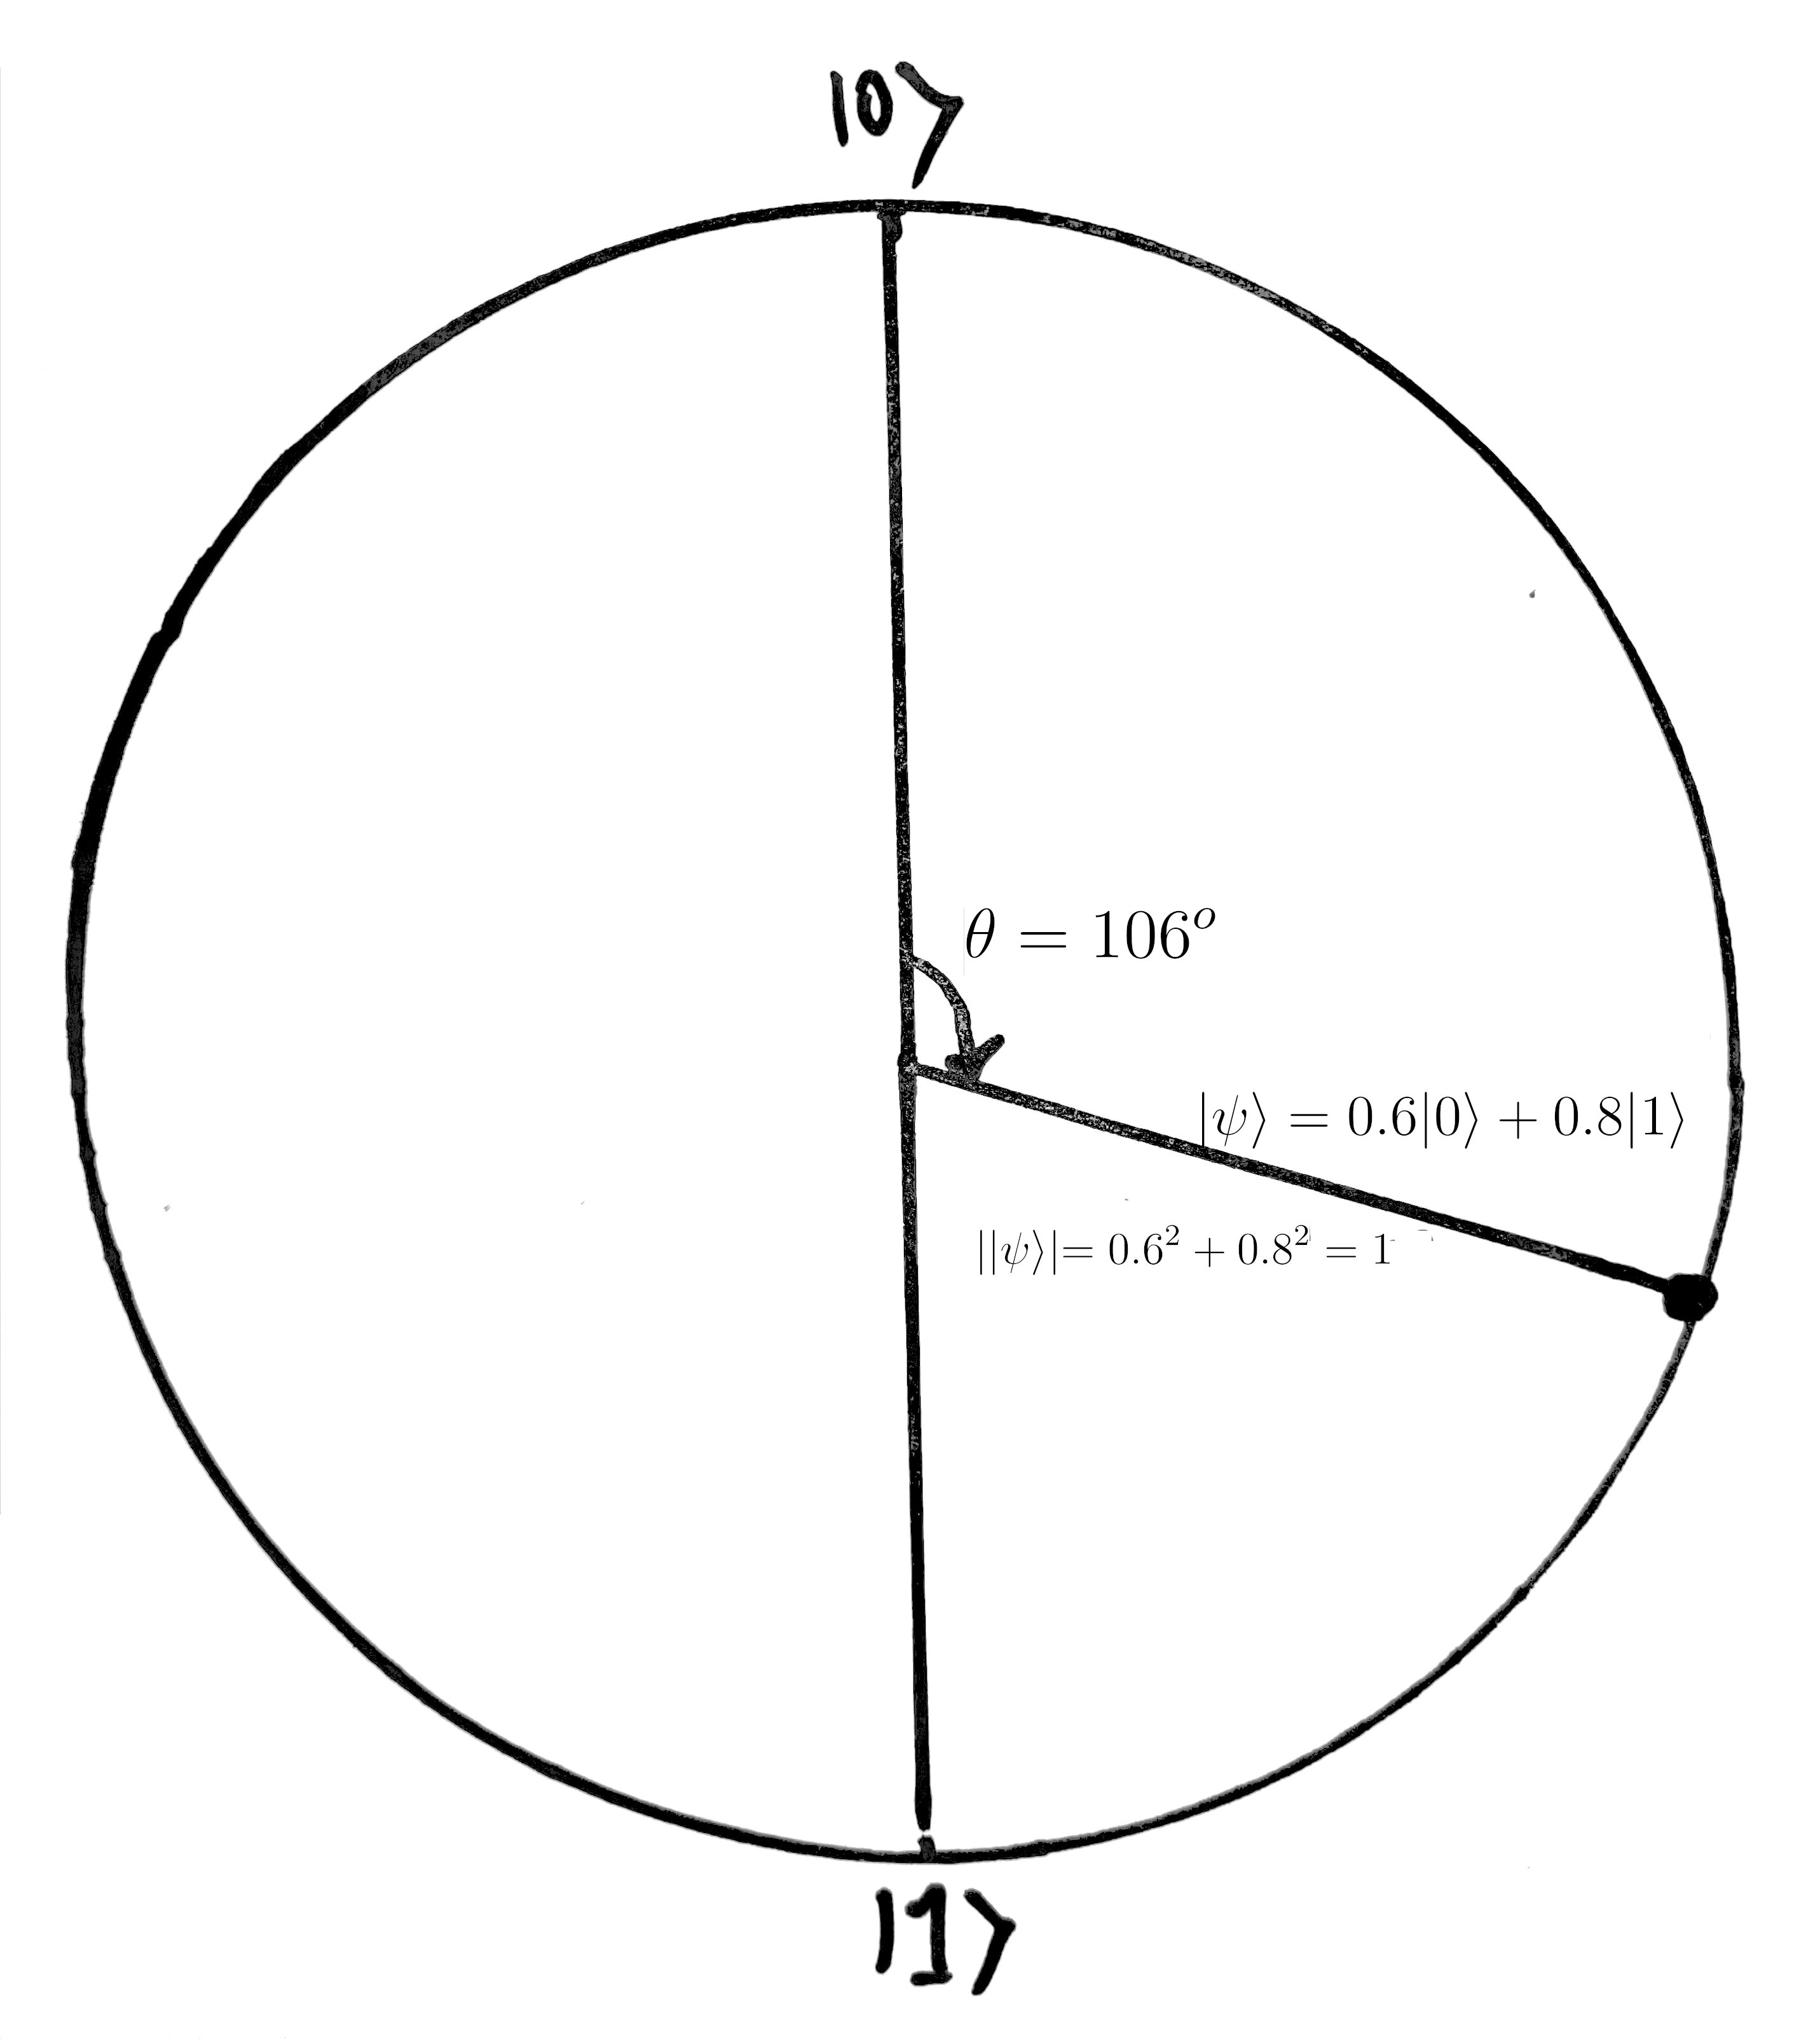
\includegraphics[width=0.5\textwidth, inner]{figures/unit-vector-2-d-hilbert-state_2.png}
	\end{adjustbox}
	\vspace{4pt}
	\caption{$\lvert\psi\rangle$ as superposition of ortho-normal bases $\lvert0\rangle$ and $\lvert1\rangle$ }
	\label{fig:2d_hilbert_space}
\end{figure}

We can in many cases think of $\alpha$ and $\beta$ as real numbers, but as they are complex numbers, 
this qubit space is described mathematically as a two-dimensional complex 
Hilbert space $\mathcal{H} : \mathbb{C}^2$ \cite{Preskill:2023} \cite{Nielsen:2010}.


%%%%%%%%%%%%%%%%%%%%%%%%%%%%%%%%%%%%%%%%%%%%%%%%%%%%%%%%%%%%%%%%%%%%%%%%%%%%%%%%%%%%%%%%%%%%%%%%%%%%%%%%%%%%%%%%%%%%%%%%
\subsubsection{Measurement \& Probability (Born rule)}

A single measurement of an $n$-qubit state yields limited information; only $n$ bits of classical data, 
are revealed. This is only a \enquote{meagre shadow} \cite{Preskill:2023} of the underlying quantum state.
So once disturbed by observation, from this quantum particle state $\lvert\psi\rangle$,
we will see it in one of these basis states, or states that we can measure and observe; 
"horizontal" or "vertical" polarization, "up" or "down" spin state, "high" or "low" energy levels.  

Whilst the system is isolated and unobserved, we can apply transforms, or computations, to the system,
and our qubit can evolve as a point on a sphere of possibilities, 
until we measure it's state as one of the two basis states.
The final measurement outcome is then inherently probabilistic; 
the probability of measuring $\lvert0\rangle$ is $\lvert\alpha\lvert^2$, or $\lvert1\rangle$ $\lvert\beta\lvert^2$.
And these co-ordinates $\alpha$ and $\beta$ have to obey certain rules, 
such as $\lvert\alpha\lvert^2 + \lvert\beta\lvert^2 = 1$; 
meaning that the final measurement of our photon guaranteed to be either "horizontal" or "vertical" polarised.

As $\lvert\alpha\lvert^2 + \lvert\beta\lvert^2 = 1$, we can effectively write our qubit state as \cite{Nielsen:2010}
$$\lvert\psi\rangle = cos \frac{\theta}{2} \lvert0\rangle + e^{i\varphi} sin \frac{\theta}{2} \lvert1\rangle $$

The numbers $\theta$ and $\varphi$ define a point on a three dimensional \emph{Bloch sphere} 
that is useful initially for visualising a qubit state.

\begin{figure}[ht] 
	\begin{adjustbox}{center}
%		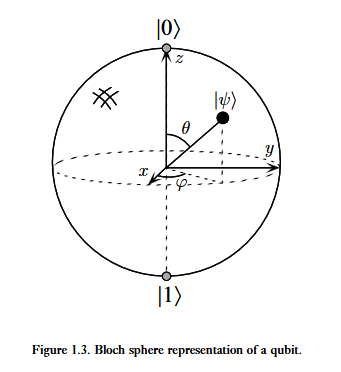
\includegraphics[width=0.5\textwidth, inner]{figures/blochsphere-nielsen-and-chuang-toc-and-chapter1-nov00.png}
		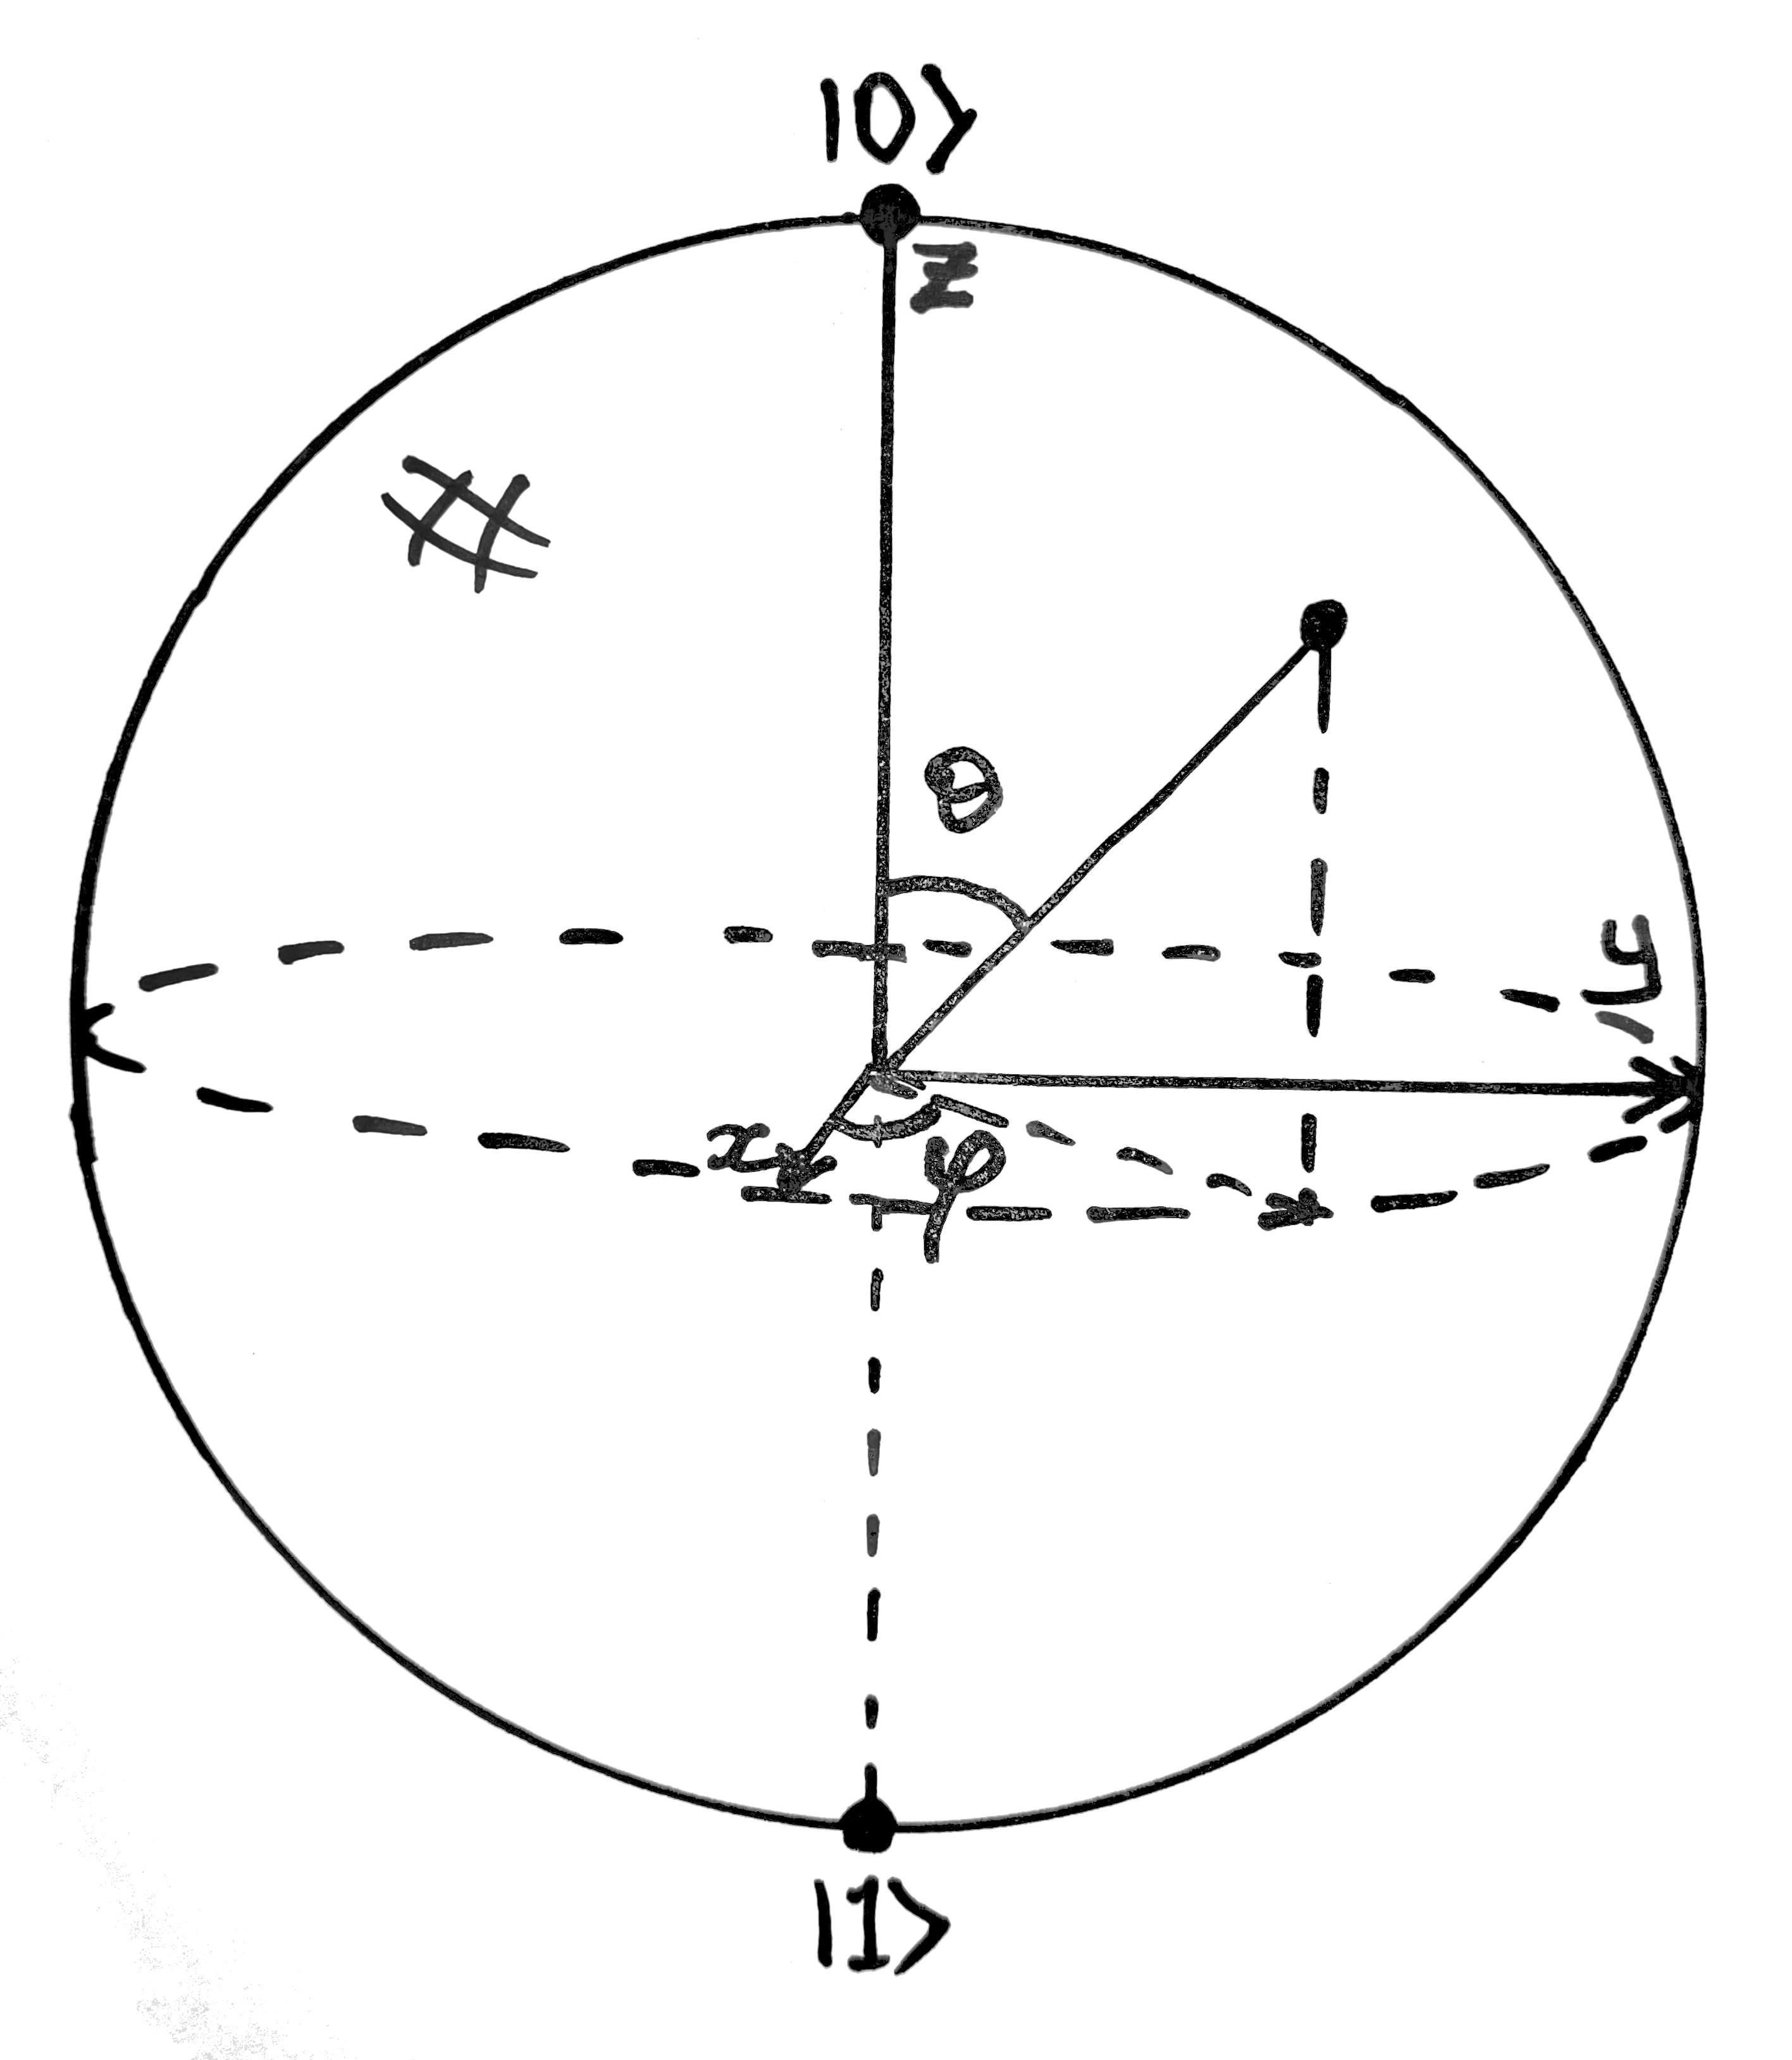
\includegraphics[width=0.5\textwidth, inner]{figures/blochsphere.png}
	\end{adjustbox}
	\vspace{4pt}
	\caption{Bloch sphere representation of a qubit}
	\label{fig:bloch_sphere}
\end{figure}

At later stages these can be developed into an understanding the benefits and difficulties each 
realisation of a quantum system.

%%%%%%%%%%%%%%%%%%%%%%%%%%%%%%%%%%%%%%%%%%%%%%%%%%%%%%%%%%%%%%%%%%%%%%%%%%%%%%%%%%%%%%%%%%%%%%%%%%%%%%%%%%%%%%%%%%%%%%%%
\subsubsection{Unitary Dynamics \& Gate Model}

We can represent the two vectors encoding these two basis states of the quantum vector space as:
$$\lvert0\rangle = \begin{bmatrix} 1 \\ 0 \end{bmatrix} \quad \textrm{and} \quad \lvert1\rangle = \begin{bmatrix} 0 \\ 1 \end{bmatrix}$$

And our qubit state can be represented as the vector:

$$\lvert\phi\rangle = \begin{bmatrix} \alpha \\ \beta \end{bmatrix} = \alpha\lvert0\rangle + \beta\lvert1\rangle$$

Postulate two of quantum mechanics (on closed-system dynamics) dictates that
an evolution of an isolated quantum system from time $t_0$ to $t_1$ is given by a \emph{unitary transformation} or operator. 
It can be shown that this is to be equivalent to applying a unitary matrix to our vector state representation \cite{Nielsen:2010}:
$$ \lvert \psi(t_1)\rangle = U \lvert \psi(t_0) \rangle$$

A matrix $U$ is unitary only if this relation with its conjugate transpose, $U^{\dagger}$ and the identity matrix, $I$, holds:
$$U^{\dagger} U = U U^{\dagger} = I$$

The conjugate transpose $U^{\dagger}$ is the inverse of U, which means that every amplitude change can be exactly undone.  
In a physical sense, we can rewind any computation:
\begin{itemize}
	\item Forward Step: $ \lvert \psi(t_1)\rangle = U \lvert \psi(t_0) \rangle$.
	\item Backward Step: $ \lvert \psi(t_0)\rangle = U^{\dagger} \lvert \psi(t_1) \rangle$.
\end{itemize}

Unitary evolution gives us \emph{reversible} computation; no information about the quantum state is lost.

This is unlike classical gates; if we take the example of a universal classical gate, 
such as the NAND gate (which can be use to construct any arbitrary logical circuit) \cite{Wikipedia:UniversalLogicGates},
we can see that given the output $1$, we cannot determine which input pair we had to begin with. 

\begin{table}[ht]
	\centering
	\begin{tabular}{ccc}
		\toprule
		$A$ & $B$ & $\text{NAND}(A,B)$ \\
		\midrule
		0 & 0 & 1 \\
		0 & 1 & 1 \\
		1 & 0 & 1 \\
		1 & 1 & 0 \\
		\bottomrule
	\end{tabular}
	\vspace{4pt}
	\caption{Truth table for a two‑input \textsc{NAND} gate}
\end{table}

%[Consider moving Toffoli example here for continuity.]
% (boolean functions can be made reversible\cite{Bennett:1989}),

%One of the postulates of quantum dynamics is that the evolution of a closed quantum system is described by a
%\emph{unitary transformation} \cite{Nielsen:2000}.  
%Given a state of a system at $t_1$ as $|\psi\rangle$, it is related to the state $|\psi'\rangle$ at time $t_2$ 
%by a unitary operator:

%$$|\psi'\rangle = U|\psi\rangle$$

%Unitary transforms are invertible by their \emph{conjugate transpose} $U^\dag$.  
%Applying the conjugate transpose, we end up where we started, 
%which is the same as applying the identity matrix $I$ to our state, leaving the state unchanged:

%$$UU^\dag = I$$

%The practical upshot is that all transforms applied to our quantum state $|\psi\rangle$ has to be a unitary transform.
%And that every tiny step in an evolving quantum system can be run backwards exactly.

From postulate 2, any valid operation on an isolated quantum system must be a reversible, information preserving,
unitary transformation, and the input state can always be reconstructed from the output, but applying the adjoint.


%%%%%%%%%%%%%%%%%%%%%%%%%%%%%%%%%%%%%%%%%%%%%%%%%%%%%%%%%%%%%%%%%%%%%%%%%%%%%%%%%%%%%%%%%%%%%%%%%%%%%%%%%%%%%%%%%%%%%%%%
\subsubsection{Tensor Products \& Circuit Construction}

In conceptualising the circuit picture of digital quantum computing, the properties of unitary matrices help us out.

The matrix product of two unitary matrices, $U_2U_1$ is also unitary, allowing us to chain gates together.

Operating on different qubits, or wires as it is helpful to think of them, we can apply gates in parallel.
This \emph{tensor}, or Kronecker product, multiplies the state space dimensions.  
Tensor-ing two small unitaries $U_1 \otimes U_2$ forms a larger block diagonal matrix \cite{Nielsen:2010}.

Put those two statements together, and we can assemble any big unitary like "Lego-bricks" from small ones;
big unitaries are just small unitaries multiplied in time and tensored in space.
And from the Solovay–Kitaev theorem, we can approximate any $2^n x 2^n$ unitary as closely as desired
using a handful of single-qubit gates and one \emph{entangling} two-qubit (e.g. CNOT) gate.
These form a \emph{universal gate set} \cite{Nielsen:2010}.


%We will define more exactly what a quantum circuit is, 
%but at this point we can understand it from the our general knowledge of classical digital circuits,
%transforming electronic states, doing our bidding in the computers that surround us in our daily lives.
%Except that we are using quantum machinery to transform quantum states.

%Because of the rules of unitary transformations, at this point, we can imagine our quantum algorithm, or circuit, 
%as one large unitary transformation, taking our initial quantum state into our desired final state.


\subsubsection{Entanglement and 'Spooky Action'}

One implication of quantum physics that troubled Einstein \cite{Einstein:1935},
in the 1935 paper \citetitle{Einstein:1935} by Einstein, Podolsky, and Rosen, 
was what is now colloquially termed \emph{spooky action at a distance} or the EPR paradox;
that two or more quantum particles can be bound into a single non-separable, or \emph{entangled} state, 
whose correlated outcomes defy classical bounds.  
The transforms effected on one particle, is tightly correlated with the state of the other.

Mathematically, entangling operations allow us to explore the full $2^n$-dimensional hilbert space
from a register of $n$ independent qubits spans; $\mathcal{H} = (C^2)^{\otimes n}$.
These entangled states cannot be represented as simple products of qubits in a superposition,
and moreover, it is entanglement that enables the constructive/destructive \emph{interference patterns}
that amplify the correct answer when we look at how Shor's and Grover's algorithms work \cite{Nielsen:2010}.

%Not all, arbitrary, transformations are valid (irreversible ones especially, and we will touch on that later)
%and an application of entanglement in super-dense coding that is a good model to covering ground quickly \cite{Nielsen:2010}

%\href{https://www.forbes.com/sites/chadorzel/2017/02/28/how-do-you-create-quantum-entanglement/}{how-do-you-create-quantum-entanglement}

%\emph{Quantum Registers}
%In quantum computing a \emph{quantum register} is a system of  \cite{Lipton:2021} (p140).

%%%%%%%%%%%%%%%%%%%%%%%%%%%%%%%%%%%%%%%%%%%%%%%%%%%%%%%%%%%%%%%%%%%%%%%%%%%%%%%%%%%%%%%%%%%%%%%%%%%%%%%%%%%%%%%%%%%%%%%%
%\subsubsection{Noise, Decoherence \& Error Correction}

%\emph{Estimating Gates and Circuit Depth}

%\emph{Note: the paper used QISKIT quantum simulator.  The paper has the shot count, but can we see the noise applied?}

%describe shot count; shot noise and statistical error-kernel variance shows up directly in OC-SVM decision boundaries.


%We recap the NISQ devices introduction from Preskill and look at error correction.

%We describe the use of logical qubits constructed from physical qubits. 

%We follow this will quantum error correction to demonstrate theoretical and practical solutions to noise and decoherence.

%Surface and colour stabiliser codes can be explained diagrammatically (hence topological protection),
% and as well as demonstrating on paper how single phase-flip and bit flip errors can be caught an corrected, 
% we can demonstrate this using SDKs.


%\subsubsection{Primitives to Support Quantum Kernel Computations}

%Now we look at the quantum kernel computation itself.  
%We are not going to analyse the 

%which often involves measurement techniques like the SWAP test, implied by overlap/fidelity calculations

The power of quantum computing is only achieved through the combination of all three phenomena:
$$ (\text{superposition})+(\text{entanglement})+(\text{interference control})$$

And students will be able to evidence this when they are introduced to :
\begin{itemize}
	\item \textbf{Superdense coding}: two classical bit of information being sent by the exchange of one entangled qubit.
	\item \textbf{Quantum teleportation}: perfect state transfer between quantum particles.
	\item \textbf{Quantum error-correction}: creating logical qubits from multiple entangled states, 
	to protect from errors from operating in noisy quantum systems.
\end{itemize}

%%%%%%%%%%%%%%%%%%%%%%%%%%%%%%%%%%%%%%%%%%%%%%%%%%%%%%%%%%%%%%%%%%%%%%%%%%%%%%%%%%%%%%%%%%%%%%%%%%%%%%%%%%%%%%%%%%%%%%%%
\subsection{Core Algorithmic Primitives}

Because of the ubiquity of Shor's algorithm for integer factorisation and finding discrete logarithms \cite{Shor:1997},
being introduced to this work gives an opportunity to understand how these ideas were generalised into methods
and building blocks that are reused across subsequent algorithms.

\begin{enumerate}[label=\textbf{\arabic*.}]
	\item \textbf{Oracle construction via modular arithmetic}\,:  
	encode classical data (e.g.\ modular multiplication or exponentiation) in a reversible, query–style unitary \(U_f\).  
	This idea separates "problem definition" from "quantum processing" and is now standard in algorithm design.
	
	\item \textbf{Unitary‐oracle abstraction}\,:  
	once the reversible black‑box \(U_f\) exists, it can be treated uniformly by
	higher-level primitives (phase estimation, amplitude amplification, QSVT,~\ldots).
	
	\item \textbf{Quantum Phase Estimation (QPE)}\,:  
	extract the eigen-phase of \(U_f\) with precision \(1/2^m\) using \(m\) control qubits; 
	QPE is the key subroutine behind order-finding,	Hamiltonian simulation, HHL and many variational routines.
	
	\item \textbf{Period finding via the Quantum Fourier Transform}\,:  
	apply QPE to the modular-exponentiation oracle to recover the period \(r\) (order) of \(a \bmod N\); 
	this is the engine of Shor's factoring and discrete-log algorithms.
	
	\item \textbf{Hidden‑Subgroup formulation}\,:  
	recast period finding as the general problem of identifying a hidden subgroup from coset states; 
	the framework unifies Shor, Simon,~etc.\ and guides research on lattice and graph‑isomorphism algorithms.
	
	\item \textbf{Amplitude Amplification (AA)}\,:  
	Grover showed that iteratively reflecting about the good and bad subspaces boosts success probability 
	from \(O(1/N)\) to \(O(1/\sqrt N)\).
	AA has since become a drop-in "quadratic booster" for search, optimisation and Monte-Carlo algorithms.
\end{enumerate}


%%%%%%%%%%%%%%%%%%%%%%%%%%%%%%%%%%%%%%%%%%%%%%%%%%%%%%%%%%%%%%%%%%%%%%%%%%%%%%%%%%%%%%%%%%%%%%%%%%%%%%%%%%%%%%%%%%%%%%%%
\subsubsection{State Preparation \& QRAM Issues}

Shor's algorithm also demonstrates the main quantum computation stages \cite{Nielsen:2010},
such as encoding classical data as a quantum state.

The problem of encoding classical data into quantum states efficiently is known to be potentially non-trverit*ivial \cite{Tavakoli:2015}, 
sometimes requiring circuits whose complexity scales with the classical data size, despite the memory compression in qubits

\subsubsection{QFT as Period Finding}

Shor implements an existing, classical, Sch\"{o}nhage-Strassen fast multiplication algorithm.
This uses a Fourier transform  to find the order of a function.  

When factoring $M = pq$, $p$ and $q$ being distinct prime numbers,
we can define a function $f_x(a) = (x^a\;mod\;M)$, which because of the modular arithmetic, is periodic.
That is, given $r' = (p-1)(q-1)$, we have $x^{a+r'}\;mod\;M = x^a\;mod\;M$, and so (because p and q are prime)  
from the Chinese Remainder Theorem, $x^{p-1} \equiv 1\;mod\;p$ and  $x^{q-1} \equiv 1\;mod\;q$.

So the function has a minimal period $r$ that divides $r'$.  
To find the smallest integer $r$ such that $x^r = 1\;mod\;M$, 
we show that $f_x(0),..., f_x(r-1)$ are distinct.  

Shor's algorithm succeeds with a probability of less than one,0
but as integer factorization is easy to verify, this is used to boost, 
or amplify the probability of success \cite{Lipton:2021}.

%%%%%%%%%%%%%%%%%%%%%%%%%%%%%%%%%%%%%%%%%%%%%%%%%%%%%%%%%%%%%%%%%%%%%%%%%%%%%%%%%%%%%%%%%%%%%%%%%%%%%%%%%%%%%%%%%%%%%%%%
\subsubsection{Amplitude Amplification}

Like many quantum algorithms, Shor and Grover demonstrate the technique which was later generalised as 
\emph{Amplitude Amplification} (AA) \cite{Dalzell:2023}.  This is the probabilistic technique of 
repeating the call and to a unitary that verifies success of the call, to boost the success probability
closer to 1.

%We have already made the point that quantum computing applies reversible unitary transformations to the quantum state.  
%The modular exponentiation arithmetic is a 

%The technique uses 
%The reversible modular exponentiation 

%So the exponential improvement of  over the classical version is 


%We can view the modular \cite{Dalzell:2023}

%%%%%%%%%%%%%%%%%%%%%%%%%%%%%%%%%%%%%%%%%%%%%%%%%%%%%%%%%%%%%%%%%%%%%%%%%%%%%%%%%%%%%%%%%%%%%%%%%%%%%%%%%%%%%%%%%%%%%%%%
%%%%%%%%%%%%%%%%%%%%%%%%%%%%%%%%%%%%%%%%%%%%%%%%%%%%%%%%%%%%%%%%%%%%%%%%%%%%%%%%%%%%%%%%%%%%%%%%%%%%%%%%%%%%%%%%%%%%%%%%
\subsection{Case-Study Back-Mapping}

In a recent paper, \citetitle{Poutre:2024}, \citeauthor{Poutre:2024} \cite{Poutre:2024} use a modified 
\emph{Large Language Model} (LLM) \emph{Transformer} auto-encoder architecture to 
\enquote{learn rich temporal limit order book subsequence representations}.  
From this trained encoder network they then train an OC-SVM to detect financial fraud, with seemingly good results.

A Support Vector Machine (SVM) is a machine learning algorithm used for classification and regression tasks.  
It is widely used in text classification and image recognition, for example.
Typically they are used in a supervised learning context where labelled data is available to fit the model.

The primary aim of the SVM is to separate data points into distinct classes by finding the best boundary that divides them.
In a 2-D space this boundary is a line, in 3-D a plane, and in higher dimensional spaces, a \emph{hyperplane}.
This boundary is found by maximising the distance between the boundary and the nearest data points in each class;
these '\emph{support vectors}' define the hyperplane. 
If the data isn't neatly separable, 
the SVM uses an mathematical transform to project the data into a higher dimensional space, 
where a clear boundary can be found.
These transformations are called \emph{kernels}, and there are many classes of kernels available.

\citeauthor{Scholkopf:1999} in 1999 \cite{Scholkopf:1999} introduced OC-SVMs as a variant of SVMs designed for one task;
outlier or novelty detection.
By focusing on distinguishing between 'normal' data and everything else, 
and only forming a hyperplane using a single class of data during training, 
they can used for semi or un-supervised applications.

\citeauthor{Kyriienko:2022} \cite{Kyriienko:2022} in 2022 developed an application of OC-SVMs using quantum kernels.
In their paper they successfully used a simulator of 20 qubits (one qubit per dataset feature)
on a reduced data set, and most interestingly, performed analysis on the training and inference times needed, 
and in the process demonstrating that the quadratic scaling of the Gram matrix evaluation 
made their approach infeasible on the full dataset.

Promising work has been done to reduce the time-complexity of the evaluation of the Gram matrix, 
by \citeauthor{Kolle:2023} \cite{Kolle:2023}, using randomised measurements and variable subsampling.

The aim of the student's paper would be to investigate whether quantum kernel OC-SVM algorithms are practical 
given our reliance of NISQ machinery.
It is well known that these devices have the constraints of having only limited number of qubit to represent model state,
and that they introduce errors that constrain the complexity and depth of circuits that they can run \cite{Preskill:2018}.
In their paper, P\"{o}utre state that their autoencoder of had a dimensionality of 128 \cite{Poutre:2024},
far larger that the feature set of 20 used by Kyriienko \cite{Kyriienko:2022}.
With the recent announcement by Google that their new 105 qubit \emph{Willow} processor has
achieved below threshold quantum error correction \cite{Google:Willow:2024}, the main body of this report is to: 
(1) reanalyse the training and inference times by Kyriienko assuming the performance stated in Google's research;
(2) assess whether the new hardware could be used to apply the OC-SVM algorithm to the P\"{o}utre paper dataset
and to estimate for the training and inference times.

Many sources emphasise the importance of "end-to-end" analysis when evaluating quantum \cite{Dalzell:2023} \cite{Morales:2025}
algorithms, including classical and quantum overheads (state preparation, measurement, error mitigation),
to assess the feasibility and potential quantum advantage of these solutions.  
Resource estimation (qubits, gates, runtimes, measurement shots) 
is a key aspect of understanding challenges and limitations,
and hence a desirable outcome for new practitioners.

%%%%%%%%%%%%%%%%%%%%%%%%%%%%%%%%%%%%%%%%%%%%%%%%%%%%%%%%%%%%%%%%%%%%%%%%%%%%%%%%%%%%%%%%%%%%%%%%%%%%%%%%%%%%%%%%%%%%%%%%
\subsubsection{Hybrid Processing Pipelines}

A second point is that details from the paper by \citeauthor{Kyriienko:2022} 
bring up an interesting point that may not be obvious from the abstract. 
Their technique is to apply only the kernel transform using quantum techniques, 
not to generate, or embed, the Gram matrix in a quantum vector state.
The constructing the Gram matrix, as well as the autoencoder, use classic computing systems. 
And as in Shor's original quantum paper on discrete logarithms and factoring \cite{Shor:1997},
this is an example of a hybrid classical-quantum computing system \cite{Preskill:2023}.

Having hands-on experience of these toolsets is a possible example of tie-ins to 
data engineering skills being developed with the full curriculum.

In this hybrid model, 
the quantum system acts as a co-processor, executing specific sub-routines that are expected to offer quantum advantage.
The classical computer orchestrates data preparation, algorithm set-up, and post-processing tasks.
There are parallels to the engineering challenges of \emph{Extract, Transform, Load} (ETL) 
in classical machine learning data pipelines and GPU workflows.

%%%%%%%%%%%%%%%%%%%%%%%%%%%%%%%%%%%%%%%%%%%%%%%%%%%%%%%%%%%%%%%%%%%%%%%%%%%%%%%%%%%%%%%%%%%%%%%%%%%%%%%%%%%%%%%%%%%%%%%%
\subsubsection{Exposure to Commercial Hybrid Pipeline Platforms}

Commercial offerings are available to support hybrid and pipelines platforms for quantum solutions.
We have options to fold practical experience into the course delivery.

Some Hybrid processing pipelines examples are:
\begin{itemize}
	\item \emph{AWS Braket Hybrid jobs}\cite{AWS:Braket:Hybrid}.
	\item \emph{Pennylane Hybrid Quantum Transfer}\cite{Pennylane:Hybrid}.
	\item \emph{Zapata Orquestra's Quantum-Enabled Workflows}\cite{Zapata:Orquestra}.
	\item \emph{IBM Qiskit Runtime Orchestration}\cite{IBM:Qiskit:Orchestration}.
\end{itemize}

%%%%%%%%%%%%%%%%%%%%%%%%%%%%%%%%%%%%%%%%%%%%%%%%%%%%%%%%%%%%%%%%%%%%%%%%%%%%%%%%%%%%%%%%%%%%%%%%%%%%%%%%%%%%%%%%%%%%%%%%
\subsubsection{Block Encoding and Quantum Linear System Solvers}

A technique that moves on from simply trying to encode classical data through a set of unitary transformations, is
%This is in contrast to Block-encoding, 
%helps define certain ideas that are needed to engage with quantum computing as $C = U_1 .. U_n$. 
the core insight that classical computing can be realised by quantum machinery, 
not by making the classical computation unitary,
but by admitting that the dynamics of a subsystem within a quantum system can be non-unitary.

The pressing problem for machine learning, Gram matrices for SVM kernels, 
Hamiltonian matrices describing a desired evolution, and general data vectors, are generally non-unitary.
If we want to run our Netflix recommender system in our brave new, fully quantum (none of this hybrid rubbish), world,
how do we keep the physics happy, whilst computing the matrix we actually want?

Without needing to understand the deeper mathematical formulation, 
there is a more advanced technique called \emph{Block Encoding} (BE) 
that can embed a, possibly non-unitary, matrix $A$ into a larger unitary $U$ \cite{Low:2017}.
And this is typically achieved by introducing additional quantum registers, or \emph{ancillas}, 

$$
U = \begin{bmatrix} A & \ast \\ \ast & \ast \end{bmatrix}
$$

An earlier foundational precursor algorithm for the technique is 
the original \emph{Quantum Linear System Solver} (QLSS) by \citeauthor{Harrow:2009} \cite{Harrow:2009}.

The history of block encoding has been detailed by Berry, Childs, Cleve, Kothari and others, 
and they show that you can simulate sparse Hamiltonians by writing them as linear combinations 
of short unitaries.

Looking at other more wide spread applications, 
there is also Quantum Singular Value Transformation (QSVT) \emph{Gilyen, Su, Low \& Wiebe} (2018),
where they apply block encoding with signal processing techniques, developing a single unifying technique.

\subsection{Justification Wrap Up}

In this section we have identified the major topic areas to include in our syllabus overview.

In the next section we collect the topics identified into subject units, with stated purposes for each topic,
and sets of learning outcomes for each unit, to guide the creation of the complete syllabus materials.